\documentclass[a4paper,10pt]{article}

\setlength{\topmargin}{-.5in}
\setlength{\textheight}{9in}
\setlength{\oddsidemargin}{.125in}
\setlength{\textwidth}{6.25in}

\usepackage{color}
\usepackage{graphicx}
\usepackage{algorithmic}
\usepackage{algorithm}
\usepackage{amsmath}
\usepackage{amssymb}
\renewcommand{\labelitemii}{$\circ$}

%opening
\title{IniMotif Manual}
\author{Lu Cheng}
\date{October 29th, 2009}

\begin{document}

\maketitle

\begin{abstract}
IniMotif devotes to discover motifs from large amounts of sequencing data.
All input sequences should be with \textbf{the same length \textit{l}}.
We also assume the existence of a \textbf{consensus sequence} (width \textit{w}) in the data.

The software is designed based on 1-base mutation Model.
At first the substring with the highest count will be chosen as the consensus sequence, then all substrings of a sequence will be compared to the consensus sequence.
The substring with the lowest hamming distance is regarded as the binding site of this sequence.
Binding sites which are 1-base mutation of the consensus sequence are used to construct the motif.

For the second motif discovery mode, the software removes \textit{l}-width sequences which contains the \textit{w}-width consensus sequence of the first run and its 1-base mutations from the input sequence pool.
Then it starts motif discovery in the same manner as that in the first motif discovery, from the rest of the \textit{l}-width sequences.
\end{abstract}



\section{Algorithm Description}
This section gives a simple description of the algorithm used by IniMotif. Here we focus on how we calculate the motif.
\begin{algorithm}
 \caption{IniMotif Algorithm}
 \label{IniMotifAlgorithm}
 \begin{algorithmic}[1]
  \STATE Initialize \textit{l}, \textit{w}, read input sequence file.
  \STATE Count all \textit{l}-width input sequences, so that we get \textit{n} unique \textit{l}-width sequences $(s_1, s_2 \ldots s_n)$ with counts $(N_{s_1}, N_{s_2} \ldots N_{s_n})$.
  \STATE Break $(s_1, s_2 \ldots s_n)$ into \textit{w}-width sbustrings (overlaping), count all the \textit{w}-width sbustrings, so that we get $(w_1, w_2 \ldots w_m)$, with counts $(N_{w_1}, N_{w_2} \ldots N_{w_n})$. \COMMENT{Identical substrings of $s_i$ are only counted once.}
  \STATE Select the \textit{w}-width substring $w_{consensus}$ with the highest count in $(w_1, w_2 \ldots w_m)$ as the consensus sequence.
  \STATE Set the mapping from binding sites to their counts $B = \varnothing$
  \FOR{$s_i \in (s_1, s_2 \ldots s_n)$}
   \IF{$s_i \ni (w_1, w_2 \ldots w_m), \, where \  d(w_i,w_{consensus}) \leq 1$}
    \STATE add $(w_1, w_2 \ldots w_m)$ to $B$, where $B(w_i) = B(w_i) + N_{s_i}/m$.
    \COMMENT{$w_i$ are all substrings with the least Hamming distance of $s_i$}
   \ENDIF
  \ENDFOR
  \STATE Set the $4 \times w$ position frequency matrix $M = \varnothing$
  \FOR{$b \in {A,C,G,T}$}
   \FOR{$j \in {1,2 \ldots w}$}
    \STATE Set $M_{bj} = B(w_{consensus}(b,j))$, where $w_{consensus}(b,j)$ is a \textit{w}-width substring by specifying the \textit{j}th base of $w_{consensus}$ as $b$.
   \ENDFOR
  \ENDFOR
  \STATE Output $M$
 \end{algorithmic}
\end{algorithm}



\section{Instructions for running the program}
The IniMotif software consists of four modules: The first java module calculates motifs and produces all necessary data;
the second matlab module draws figures from the data produced by the first module;
the third perl module draws logos for all produced motifs;
the fourth perl module organizes all information in the form of HTML pages.
We strongly recommend you to read Section \ref{sec:techspec} if you are not clear about the predefined specifics.


\subsection{The java module}

\begin{itemize}
\item How to run the module? \\
cd IniMotifDirectory \\
make compile \\
java -jar InitialMotif.jar \textcolor{red}{-MODE} [-skip] \\
\# In case of low memory, please use ``java -Xms4g -Xmx4g -jar InitialMotif.jar \textcolor{red}{-MODE}'' instead 

\item Different Modes \\
the ``\textcolor{red}{-MODE}'' can be replaced by the following parameters:
\begin{itemize}
 \item -uniform: the input directory contains all barcode files of all cycles and all batchs in one folder, only the primary motifs will be calculated
 \item -secondary: the input directory contains all barcode files of all cycles and all batchs in one folder, both the primary and secondary motifs will be calculated
\end{itemize}

\item ``-skip'' option \\
the ``-skip'' option enables one to skip processing data that has already been processed, it is useful when new sequence files are added to the input directory.
For a sequence file, IniMotif checks whether the necessary data files are available in the corresponding output directory. If all data files are available, then this sequence file will not be processed.

\item Parameter setting (in paras/para.txt)
\begin{itemize}
 \item line 1: Description of the parameters
 \item line 2: the input directory (includes sequence files of all batches and all cycles)
 \item line 3: the output directory
 \item line 4: the location of the background distribution file
 \item line 5: the location of the barcode-TfName table file \verb+(fullbarcode \t TfName)+
 \item line 6: the minimum motif width
 \item line 7: the maximum motif width
 \item line 8: the length of the input sequences
\end{itemize}

\item Other settings
\begin{description}
 \item[Background base distribution] Background base distribution is set in BackDis.txt, in the order of A, C, G, T. It is 
                                     suggested to be estimated from the original batch (batch `0').
 \item[SELEX experiment Setting] The Well\_Plate\_Barcode.txt files contains the mappings between (well, plate) and barcode.
                                 The elements of each line are seperated by tab, i.e. \verb+\t+.
\end{description}

\item Function explaination \\
After producing necessary data, the java module will call Matlab module to produce the data, then call the perl module for drawing logos,
finally it calls the perl module to produce HTML files. The commands will be shown in the STDOUT. The matlab module will produce ``.png'' figures by default. \textbf{Note}: the sequence data of the background batch (batch `0') should always be included in the input directory.

\end{itemize}


\subsection{The matlab module}

\begin{itemize}
\item How to run the module? \\
\verb+cd IniMotifDirectory/CreateFigure+ \\
\verb+matlab &+ (graphical mode) OR \verb+matlab -nodisplay+ (non-display mode) \\
\verb+drawAllBatches(root_dir, widths, MODE, FIGURE_TYPE)+
  \begin{description}
   \item \verb+root_dir+ : The root directory is the directory which contains data for all batches, \\ i.e. \mbox{`IniMotifOutput'} or `SecondMotif'.
   \item \verb+widths+ : Prespecified motif widths, [6:10] means width 6 to 10, [8:8] means width 8
   \item \verb+MODE+ : \verb+`normal'+ for producing new figures, \verb+`skip'+ for skipping already existed figures
   \item \verb+FIGURE_TYPE+ : Figure format of matlab output figures, `png' or `ps'. By default it is set as `png'.
   \item \textbf{An example}: \verb+drawAllbatches(`selex/IniMotifOutput', [6:10], `skip', `png')+
  \end{description}

\item Useful function-1: \verb+drawOneCycle(CYCLE_DIR, WIDTH)+ \\
This function draw SubStrCount-HamDisFig and PosDisFig under one cycle
directory. \texttt{CYCLE\_DIR} is the directory of one cycle, which includes processed data
for all different widthes, \texttt{WIDTH} specifies the widths under this cycle directory.

\item Useful function-2: \verb+drawTrendFig(batch_dir,back_dir,WIDTH,out_dir)+ \\
This function draws the TrendFig for all barcodes under one batch directory.
The batch directory contains different cycles \texttt{batch\_dir} is the directory of the batch for drawing the Trend figure.
\texttt{back\_dir} is the directory of the initial cycle, i.e. \texttt{`IniMotifOuput/0/0'}. 
\texttt{WIDTH} should be an integer here, \texttt{out\_dir} specifies the output directory for the trend figures.

\end{itemize}


\subsection{The perl module}
This module contains two parts: the first part for drawing logos and the second part for producing HTML pages.
\begin{itemize}
 \item \textbf{Logo construction} \\
   \texttt{cd IniMotifDirectory/CreateLogo} \\
   \texttt{perl drawAllLogo.pl -NORMAL . IniMotifOutputDir [skip]} \\
   This command produces logos for all motifs files in the output, where \\
   \texttt{IniMotifOutuputDir} is the output directory of IniMotif, i.e. directory contains all outputs; \\
   \texttt{skip} will not process a motif file if a logo already exists

 \item \textbf{HTML construction} \\
   \texttt{cd IniMotifDirectory/HTML} \\
   \texttt{perl genPages.pl . IniMotifOutputDir minWidth maxWidth} \\
   This command creates all HTML pages for organizing the data, where \\
   \texttt{IniMotifOutuputDir} is the output directory of IniMotif, i.e. directory contains all outputs;\\
   \texttt{minWidth, maxWidth} mean the minimum and maximum motif widths, respectively.

 \item \textbf{A useful script} \\
   Sometimes we want to view the results in another computer, but the results are quite huge. Thus it is useful if we just extract the figures and HTML pages. \\
   \texttt{cd IniMotifDirectory/HTML} \\
   \texttt{perl downloadPages.pl IniMotifOutputDir downloadDir} \\
   The above commands download all necessary figures and HTML files for visualization, where \\
   \texttt{IniMotifOutuputDir} is the output directory of IniMotif, i.e. directory contains all outputs;\\
   \texttt{downloadDir} is the directory for storing the figures and HTML files.\\
\end{itemize}

\section{Result Description}
\label{sec:resultdescription}
This section explains all the files under the WIDTH directories, which are the most basic unit folders in the IniMotif output directory. 
Our default directory are these WIDTH directories. Here we use \texttt{fullbarcode} to represent any legal full barcode, and \texttt{barcode} to
 represent the central part of a \texttt{fullbarcode}.

\subsection{Motif \& logo}
The \texttt{fullbarcode}.pwm (in motif folder) files show the motif information.
The first line gives \texttt{fullbarcode} and its corresponding TF name.
The following two lines are the consensus sequence and its reverse complement, followed by the count of the consensus sequence.
Then the Alignment matrix, Frequency matrix, Information content-based weight matrix (for calculating free binding energy) are given.
Finally the logo matrix for drawing the logo and the background base distribution are provided.

The \texttt{fullbarcode}.png files (in logo fodler) show the logos drawn from the logo matrixes in the corresponding \texttt{fullbarcode}.pwm motif files.
The title of logo consists of the \texttt{fullbarcode} and its corresponding TF name. 

\subsection{SubStrDis}
\texttt{fullbarcode}.cnt files in this folder provide the counts of the each \textit{w}-width substring (overlapping) in the original sequence files.
The .cnt files are used for drawing the substring changing trend figures.
The first column are the indexes of each \textit{w}-width substring;
The second column are the counts of each \textit{w}-width substring.
Note that the count of each \textit{w}-width substring (exclude palindrome) is the sum of this substring and its reverse complement.
If the count of a \textit{w}-width substring is less than 3 or 1/10 of the expected number of a random sequence, it will not be recorded in the .cnt file

\subsection{SubStrDis-HamDis \& SubStrDis-HamDis-Figure}
The \texttt{fullbarcode}.dat files (in SubStrDis-HamDis folder) provide data for drawing the \texttt{fullbarcode}.png files in the SubStrDis-HamDis-Figure files.
\begin{itemize}
 \item Structure of \texttt{fullbarcode}.dat \\
 The first row shows the fullbarcode and TF name.
 Each of the following rows represents a \textit{w}-width substring, which is counted from each \textit{w}-width substring with
 the least Hamming distance to the consensus sequence on each \textit{l}-width sequence in the input sequencing file.
   \begin{itemize}
    \item The first column labels a substring. A subtring with higher Hamming distance than its reverse complement with labeled as 1; otherwise it is labeled as 0.
    \item The second column is the count of this \textit{w}-width substring, note that it is not the sum of both strands this time
    \item The third column shows the Hamming distance to the consensus sequence
    \item The fourth column is the index of the substring
   \end{itemize}

 \item Explanation of the SubStrCount-HamDis figure
   \begin{figure}[htp]
    \centering
    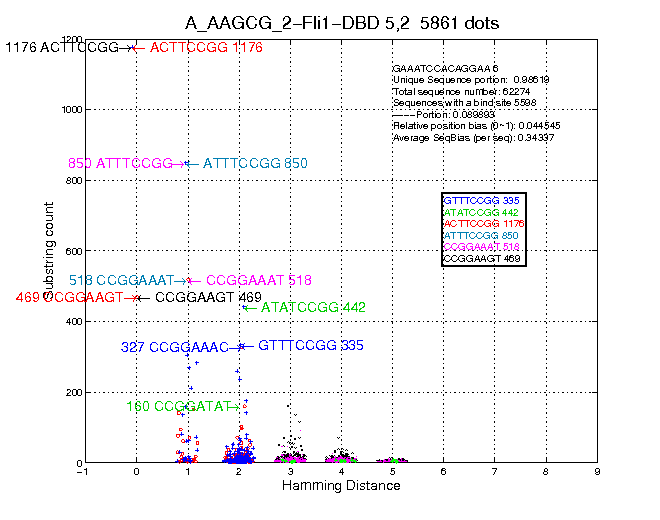
\includegraphics[width=0.7\textwidth]{A_AAGCG_2.png}
    \caption{SubStrDis-HamDis-Figure}
    \label{fig:subhamfig}
   \end{figure} \\
  As shown in \figurename{} \ref{fig:subhamfig}, the title shows the fullbarcode of TF \texttt{Fli1} is \texttt{A\_AAGCG\_2},
  and the total number of dots in this figure is 5861. Each dot in the figure is a 8-width 'binding site', 
  i.e. the 8-width substring with the least Hamming distance to the consensus sequence among all 8-width substrings of a 14-width sequence. 
  The X value of a dot is the Hamming distance to the consensus sequence; the Y value of the dot is the count of the 'binding site' in all the
  14-width sequences of the input sequence file. Note that some variations of the position have been added to the dots for better visualization.
  The sequences with Hamming distance 0 should be the consensus sequences, one of which is the reverse complementary sequence of the other.
  The text on the up-right corner shows the 14-width sequence with the highest count, followed by the portion of unique 14-width sequences. 
  There are 62274 sequences (14bp) in the input file, 5598 of which contain a binding site. 
  The relative position bias shows the bias for location of the 8-width binding sites on the 14-width sequences.
  The `Average SeqBias' shows the average sequencing bias (See Section \ref{sec:seqbias}).
\end{itemize}


\subsection{BindSitePosDis \& PosDis\_Figure}
The \texttt{fullbarcode}.dis files (in BindSitePosDis folder) contain other information besides data for drawing \texttt{fullbarcode}.png files under PosDis\_Figure.
\begin{itemize}
 \item The \texttt{fullbarcode}.dis file structure
  \begin{itemize}
   \item Row 1: the \textit{l}-width sequence with the highest count in the input sequencing file.
   \item Row 2: the count of the highest \textit{l}-width sequence
   \item Row 3: the proportion of unique sequences in the input sequencing file
   \item Row 4: the total number of \textit{l}-width sequences in the input sequencing file
   \item Row 5: binding site position distribution on the forward strand
   \item Row 6: binding site position distribution on the reverse strand
  \end{itemize}

 \item Explanation to binding site position distribution figures
   \begin{figure}[htp]
    \centering
    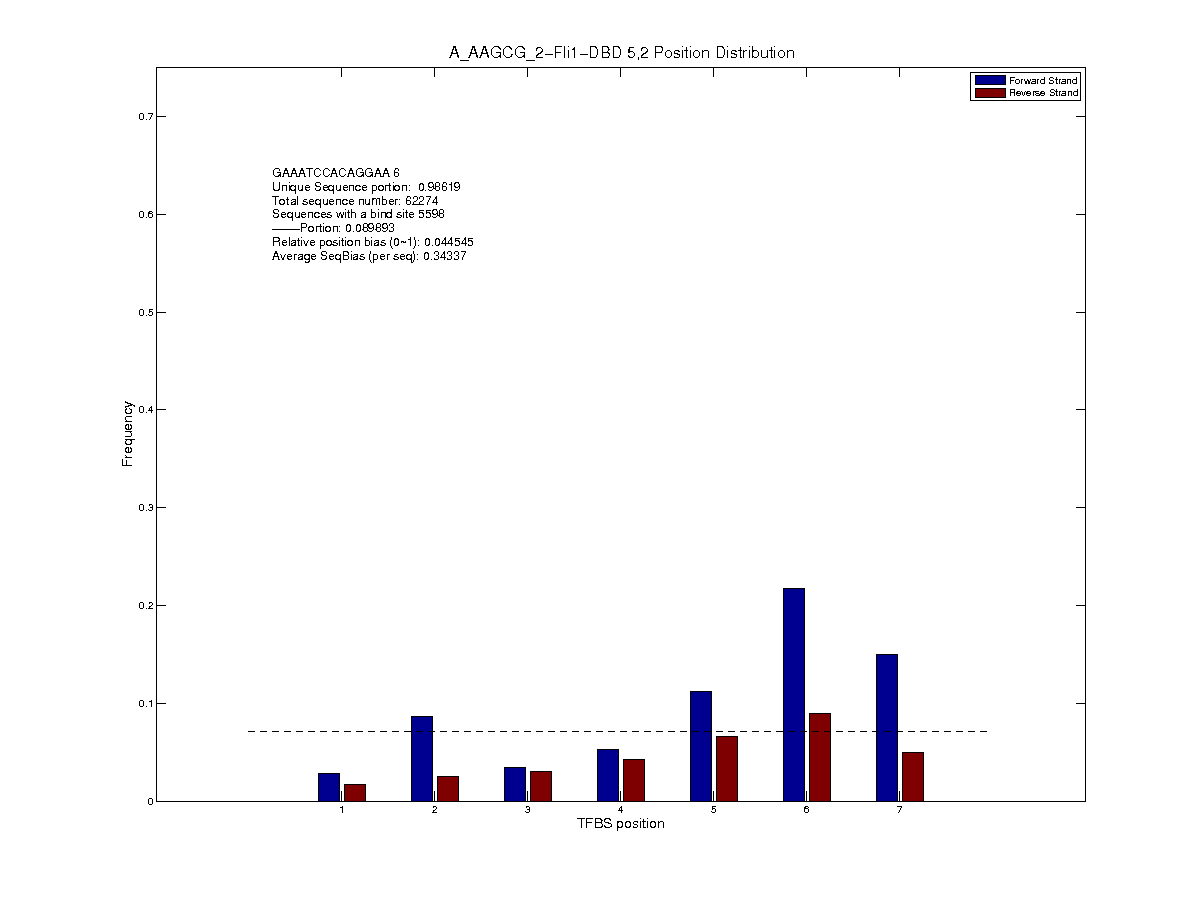
\includegraphics[width=0.8\textwidth]{A_AAGCG_21.png}
    \caption{SubStrDis-HamDis-Figure}
    \label{fig:posdisfig}
   \end{figure} \\
 As shown in \figurename{} \ref{fig:posdisfig}, the blue and red bars shows the position distribution of the binding sites.
 The distribution is normalized over all postions on both forward and reverse strands.
 The dashed line means the uniform distribution.
\end{itemize}

\subsection{SeqBias}
\label{sec:seqbias}

\begin{itemize}
 \item Definition of SeqBias \\
  The \texttt{fullbarcode}.bias files under the SeqBias provide information of the sequencing bias.
  Since DNA is a double strand, we have equal chance to sequence both strands.
  This equality is supposed to be shown in our data. 
  But in real cases, the numbers of substrings on one strand differ a lot from the other. 
  We use seqbias to indicate the difference.
  Here we denote all \textit{w}-width substrings as A, and the count of a random substring s in A as Count[s].
  The following formula calculates the average sequencing bias.
  \begin{equation}
   \textit{seqbias(s)} = \frac{ \sum_{s \in A} \left| Count[s] - Count[RevCom(s)] \right| }{ \sum_{s \in A} \left| Count[s] + Count[RevCom(s)] \right| } 
                       \approx \frac{\bar{p}-\frac{1}{2}}{\frac{1}{2}}
  \end{equation}
  where the $\bar{p}$ is the average proportion of a substring in the data.
  This formula tells how biased the sequencing is from equal equal sequencing state.
  If both strands are equally sequenced in the data, then there is no bias, which means the value of the formula is 0.
  If only one strand is sequenced, the value of this formula is 1, which means maximum bias.
  By experience, if the sequencing bias exceeds 0.5, we think there exists large sequencing bias in the data and needs further investigation.

 \item Structure of \texttt{fullbarcode}.bias file \\
  The first row is the \texttt{fullbarcode} and TF name;
  The following rows show counts of each \textit{w}-width substrings and its reverse complement in the input sequencing files.
  Note that if both counts of a \textit{w}-width substrings and its reverse complement are smaller than 5 or 1/10 of the expected number of a random \textit{w}-width substring, the \textit{w}-width substring will not be recorded.
 
\end{itemize}



\section{TrendFig}
This section gives a simple introduction to the substring trend changing figures.
  \begin{figure}[htp]
   \centering
   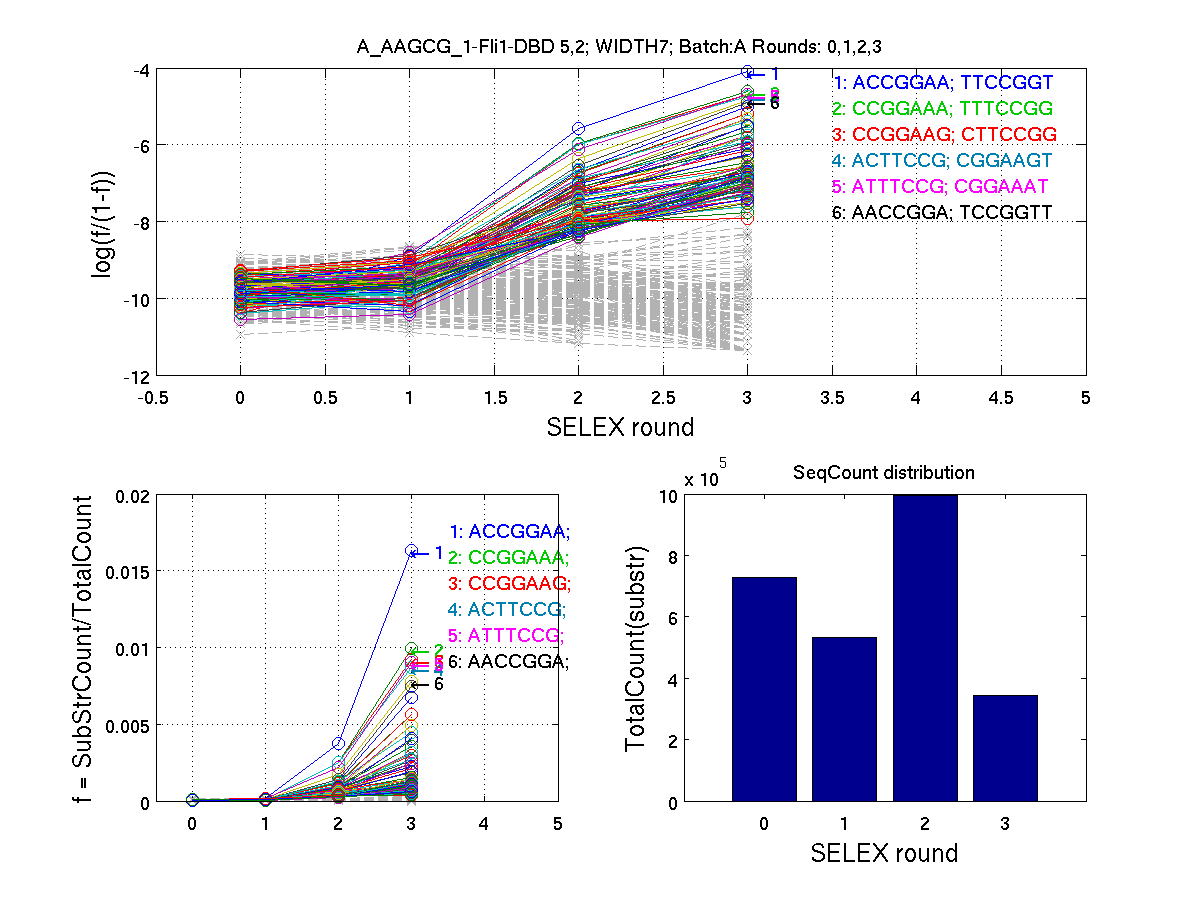
\includegraphics[width=0.8\textwidth]{a.png}
   \caption{Substring trends}
   \label{fig:trendfig}
  \end{figure} \\
We count all the 7-width substrings (overlapping) of the input 14-width sequences.
Identical repetitive 7-width substrings within one 14-width sequences are excluded.
Then the substring counts are normalized to the total substring count.
The portion of each 7-width substring is represented as $f = SubStrCount/TotalCount$, as shown in the lower left part of the figure.
For better illustration, we also plot the relative portion of each 7-width substring, as shown in the upper part of the figure.
Each line in the above figure represents a substring. 
Top 100 substrings (in different colors) with the highest average counts over all selex rounds, 
and 200 substrings (grey dashed line) randomly selected from all substrings are shown in \figurename{} \ref{fig:trendfig}.
The title includes TF names, barcode, width, and cycles used to construct this figure.
The bars show the total count of substrings in each round.
To produce the trend figure, the substring distribution of the initial pool (cycle 0) needs to be specified.



\section{HTML pages}
The HTML pages are quite easy to read.
The only difficult part is the \texttt{CONSENSUS\_1} and \texttt{CONSENSUS\_2} in the index page.
\texttt{CONSENSUS\_1} means the 8-width consensus sequence (SELEX cycle 3) in the first run of motif discovery.
\texttt{CONSENSUS\_2} means the 8-width consensus sequence (SELEX cycle 3) in the second run of motif discovery.
When the 8-width consensus sequence of cycle 3 is not avaiable, \texttt{`NNNNNNNN'} will be used. 
The size of images can be set in \texttt{barcode.css} file. Also \texttt{Ctrl++} and \texttt{Ctrl--} are used to zoom out/in for viewing the HTML pages.



\section{Technical specifics}
\label{sec:techspec}
This section introduces the specifics of the IniMotif software.


\subsection{Full barcode structure}
The \texttt{fullbarcode} looks like: \verb+0_ACGTC_0, A_ACGTC_3+ \ldots \\
The first part shows the sequencing batch; the central part is the barcode; and the last part is the
selex cycle.
Here we use the regular expression to represent the full barcode: \verb|[0A-Z][A-Z]*_[A-Z]+_[0-9]+|.


\subsection{Hierarchy of Input and output}
\figurename{} \ref{fig:outputhierachy} shows the hierarchy of input and output. \\
  \begin{figure}[htp]
   \centering
   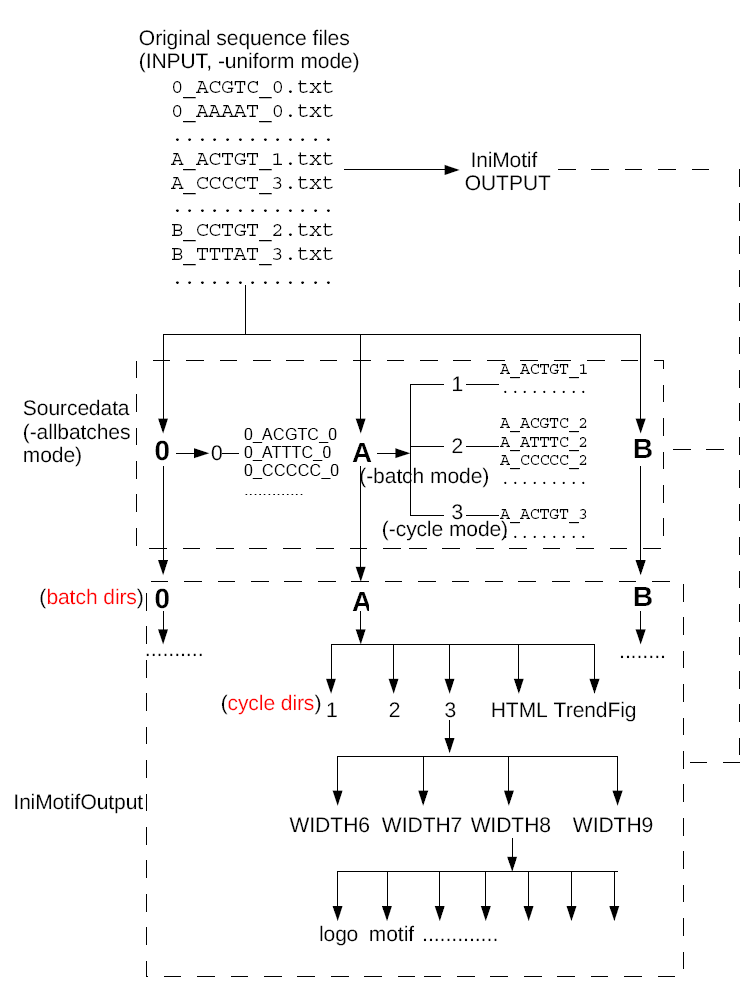
\includegraphics[width=0.7\textwidth]{HAHA2.png}
   \caption{Hierachy of IniMotif Output}
   \label{fig:outputhierachy}
  \end{figure}

We assume all input sequences files are placed in one folder. 
Then the sequences files are separated into different subfolders according to their batches and cycles, as shown in the 'sourcedata' folder.

The output of IniMotif is organized the same way as the input. 
The top level is the batch folders, then there are cycle folders under the batch folders, under the cycle folders, the data are organized according to motif widths.
For the contents in the width directories, please refer to Section \ref{sec:resultdescription}.


\subsection{Organization of the background distribution file \texttt{BackDis.txt}}
The background distribution file \texttt{BackDis.txt} tells the frequencies of \texttt{`ACGT'} in the initial SELEX pool.
It should be one line file which consists of 4 numbers between 0 and 1, whose summation should be 1.
The numbers are tab separated.


\subsection{Organization of the \texttt{Barcode-TfName.txt} file}
This file constructs the mapping from fullbarcode to TF names.
This file contains two columns.
The first column should contain the fullbarcode, the second column are their corresponding TF names.
The columns are tab separated.


\subsection{Organization of the \texttt{Well\_Plate\_Barcode.txt} file}
This file constructs the mapping from barcode to (plate, well) of SELEX experiments.
Note that we use barcode here, which is the central part of the full barcode.
This file contains three columns. 
The first column shows the well of a SELEX experiment; the second column is the plate; the third column is the barcode.
The columns are tab separated.



\section{Implementation details}
There exist many implementation details, this section lists the most importants ones.
\begin{itemize}
 \item When calculating the consensus sequence, identical substrings of a \textit{l}-width sequence will only be counted once
 \item When calculating the consensus sequence, both a \textit{w}-width sequence and its reverse complements will be counted (except palindrome)
 \item When searching \textit{w}-width binding sites on a \textit{l}-width sequence, first all substrings with the least Hamming distance are picked; then if the least Hamming distance is less than 2, the picked substrings are chosen as binding sites; finally the count of the \textit{l}-width sequence is averaged over all chosen binding sites, as the count of each binding site. Thus you may see 0.5 sequences in the final position frequency matrix.
 \item When producing data for SubStrCount-HamDis figure, substrings with counts less than a threshold (here we set as 3) are not included.
 \item When producing data for TrendFig, if both counts of a substring and its reverse complent are less than a threshold (here we set as 3), the substring will be discarded.
\end{itemize}



\section{Dependencies of IniMotif}
\begin{itemize}
 \item Operation System: Linux
 \item Java, JDK 1.5
 \item Perl 5.0
 \item Perl, TFBS module (http://tfbs.genereg.net/)
 \item Matlab 7.0
\end{itemize}



\section{Limitations}
This section gives a simple description of the limitations of IniMotif.

All sequences used in this program should be shorter than 31bp.

For a width 12-16 motif discovery task from $2,000\sim50,000$ 20bp sequences, 
apporximatedly 4g mememory is needed for the java module, 
2g memeory is needed for the matlab module, 
and 1g is needed for the logo and HTML pages construction.

Please contact \texttt{lu.cheng.cs@gmail.com} if there is any problem.

\end{document}
